\documentclass[10pt,a4paper]{article}
\usepackage[utf8]{inputenc}
\usepackage{amsmath}
\usepackage{amsfonts}
\usepackage{amssymb}

\usepackage{graphicx}

\usepackage[ngerman]{babel}
\usepackage{epstopdf}

\usepackage{fancybox}

\usepackage[left=1cm,right=1cm,top=1cm,bottom=1cm]{geometry}
\title{Asymmetrische Kryptographie in Java\\Handout}
\author{A. H. W. Lindemann, N. Vetter}
\date{10. Januar 2014}

\begin{document}
\maketitle
\section{Asymmetrische Kryptographie}
\subsection{Kerckhoffs Prinzip}
\begin{center}
\Large
\shadowbox{\glqq Sicherheit ist allein vom Schlüssel und nicht vom Verfahren abhängig.\grqq}
\end{center}

\subsection{Theorie}

$\Rightarrow$ Einwegfunktionen mit Falltür.
\begin{itemize}
\item injektive Funktion $f:X \rightarrow Y$
\item $\forall x \in X$ ist f(x) effizient zu berechnen
\item aus Bild y = f(x) darf Urbild x nur \glqq effizient\grqq ~berechnet werden können, wenn Zusatzinformationen verfügbar sind.
\item Bsp.: h-te Potenz mod(n), Zusammengesetzter mod(n)
\end{itemize}

\begin{figure}[ht]
\begin{minipage}[c]{0.60\linewidth}
\centering
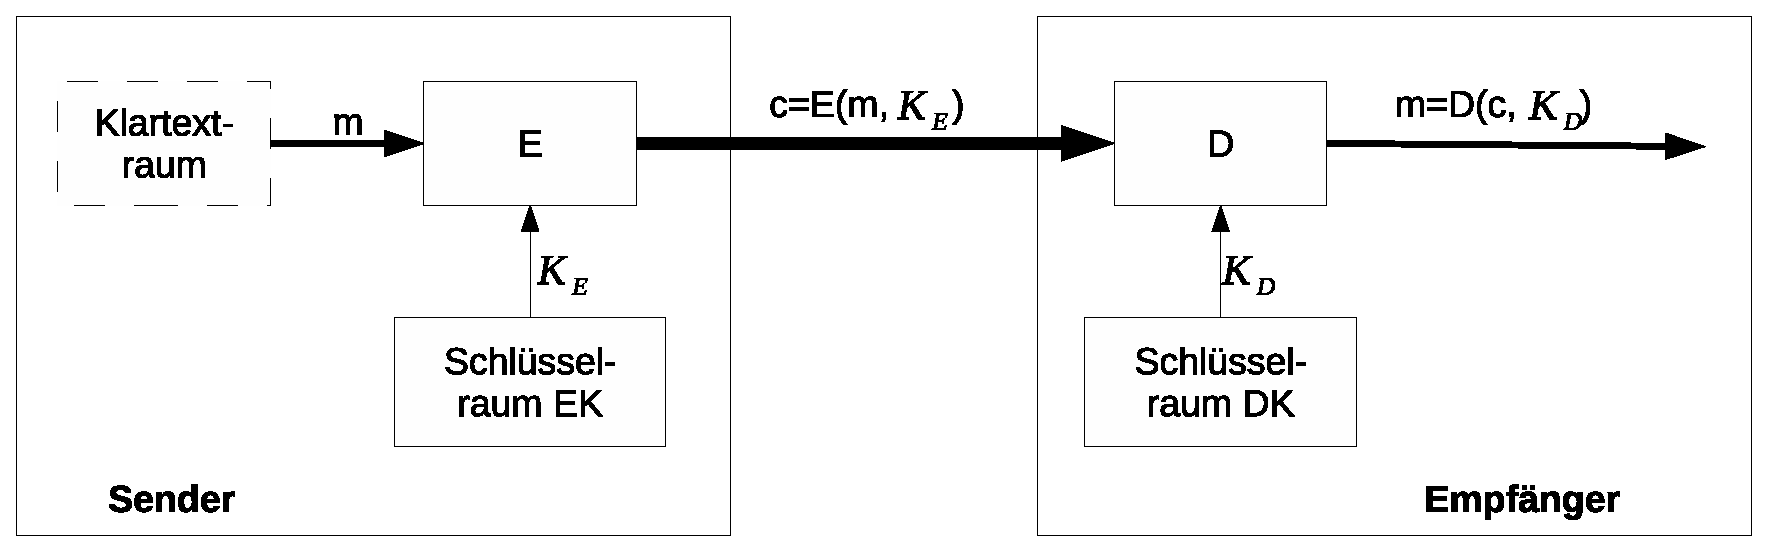
\includegraphics[width=\textwidth]{async.eps}
\caption{Asymmetrische Kryptographie (nach \cite{Eckert13})}
\end{minipage}
%\hspace{0.5cm}
\begin{minipage}[c]{0.40\linewidth}
\centering
\small
\begin{itemize}
\itemsep0pt
\item Tupel = ($M,C,EK,DK,E,D$)
\item 2 endliche Alphabete ($A_1,A_2$)
\item Klartext ($M \subseteq A^*_1\backslash\emptyset$)
\item Kryptotext ($C \subseteq A^*_2\backslash\emptyset$)
\item Verschlüsselungsschlüsselraum ($EK\backslash\emptyset$)
\item Entschlüsselungsschlüsselraum\\
($DK/\emptyset~mit~f:EK \rightarrow DK ~und~ f(K_E)=K_D)$
\item Verschlüsselungsverfahren ($E :~ M x EK \rightarrow C$)
\item Entschlüsselungsverfahren ($D :~ C x DK \rightarrow M$)
\item Es gilt: $\forall M : D(E(M,K_E),K_D) = M$
\end{itemize}
\end{minipage}
\end{figure}

\subsection{Vertreter}
\begin{itemize}
\item RSA, DSA, Diffie-Hellman, ElGamal
\end{itemize}

\subsection{Anwendungen}
\begin{itemize}
\item PGP, SSL / TLS
\end{itemize}

\newpage
\section{Hybride Kryptographie}
\begin{figure}[hbtp]
\centering
\includegraphics[width=\textwidth]{hybrid.PNG}
\caption{Hybride Kryptographie (Alice $\rightarrow$ Bob, aus VL "`Sicherheit in Rechnernetzen"')}
\end{figure}

\begin{figure}[!ht]
\begin{minipage}[t]{0.45\linewidth}
\centering
\begin{itemize}
\item Nachricht = $m$
\item Komprimierung = $Z$
\item Verchlüsselung = $E$
\item symmetrischer Schlüssel = $K_S$
\item öffentlicher Schlüssel (Bob) = $K_B$
\end{itemize}
\end{minipage}
\hspace{0.5cm}
\begin{minipage}[t]{0.45\linewidth}
\centering
\begin{itemize}
\item Konkatenation = $||$
\item verschlüsselter symmetrischer Schlüssel = $E(K_S)$
\item Entschlüsselung = $D$
\item privater Schlüssel (Bob) = $K_B ^{-1}$
\item Dekomprimierung = $Z^{-1}$
\end{itemize}
\end{minipage}
\end{figure}

\section{Java-Implementierung}
\subsection{JCA vs JCE}
Abspaltung aufgrund von Exportbeschränkungen der USA:
\begin{itemize}
\item \textbf{J}ava \textbf{C}ryptography \textbf{A}rchitecture - Hashfunktionen, Schlüsselgeneratoren,...
\item \textbf{J}ava \textbf{C}ryptography \textbf{E}xtension - Verschlüsselungsfunktionen
\end{itemize}

\subsection{Kryptoprovider}
\begin{figure}[!ht]
\begin{minipage}[t]{0.45\linewidth}
\centering
Interne Provider\\
Beispiel "`The SunJCE Provider"'
\begin{itemize}
\item AES, DES, ...
\item RSA
\item Diffie-Hellman
\end{itemize}
\end{minipage}
\hspace{0.5cm}
\begin{minipage}[t]{0.45\linewidth}
\centering
Externe Provider\\
Beispiel "`Bouncy Castle"'
\begin{itemize}
\item AES, DES, ...
\item RSA, ElGamal, NTRU
\item Diffie-Hellman (verschiendene Varianten)
\end{itemize}
\end{minipage}
\end{figure}


\section{Literaturliste}
\nocite{Eckert13}
\nocite{Engelbrecht04}
\bibliography{literatur-Java-Security}{}
\bibliographystyle{apalike}
\end{document}
